\section{Introduction}\label{sec:intro}
zbMATH classified more than 
\href{https://zbmath.org/?q=%2A+py%3A2019}%
{80k} articles in 2019 according to the Mathematical Subject Classification~(MSC).
With more than
\href{https://msc2020.org}%
{5000} class labels, this classification task requires significant depth-knowledge of the particular fields of mathematics in order to obtain correct fine-grained classifications of the articles.
Therefore the classification procedure is two-fold.
At first, the articles are pre-classified into one of \href{https://msc2020.org}%
{63} main classifications, which are the two first digits of the first MSC label of each article.
In a second step, domain expert assigns fine-grained classification labels in their area of expertise.

In this paper, we focus on the coarse-grained classification and explore how modern machine learning technology can be employed to automate this process.
In particular, we compare the current state of the art technology with a system customized for the application in zbMATH from 2014~\cite{SchonebergS14}.
We formulate the following research questions:
\begin{enumerate}
  \item Which measures are appropriate to assess the quality of automatic classifications?
  \item Does the inclusion of mathematical formulae improve the quality of the classifications?
  \item Does the Part of Speech (POS) preprocessing improve the quality of classifications?
  \item Which features (Title, Abstract, References) are most important for the correct classification?
  \item How does the quality of automatic classification compare to manual classifications?
  \item How to avoid misclassifications in the future?
  \item How can the best performing method be integrated into the current production pipeline at zbMATH?
\end{enumerate}
\section{Method}\label{sec:method}
To investiagte the given problem, we first create a test and training dataset, second we investage different encodings, train our models and evaluate the results.
\subsection{Generation of a test and training dataset}
\paragraph{Filter current high quality articles}
The zbMATH database has assiged MSC classes to more than
\href{https://zbmath.org/?q=cc%3A*}%
{3.6M} articles.
However, the way how mathematical articles are written changed in the last century.
Therefore, we did focus on recent articles from the years 2000 to 2019 and limited ourseles to selected yournals.
Moreover, we restricted ourselves to articles in english and limited ourselfes to abstracts rather than reviews of articles.
To be able to compare methods that are based on references and methods that use text and title we only selected articles that have one reference that
can be matched to another article.
In addition we excluded articles that are not finally published and processed and thus do not yet have a zbl-number.
\paragraph{Splitting to test and training set}
After applying all these filters, we split the resulting list of 442'382 articles into a test and training set.
For the test set it was important to us that we can also measure the bias of our zbMATH classification labels.
Therefore, we used the articles of which we knew the classification by the MR service as training set.
The resulting training set consists of $n=32'230$ articles and the training set of 410'152 articles.
To ensure that these selection does not introduce additional bias, we did also compute standard 10 fold cross validation.
\paragraph{Definition of article data format}
To maximize rerproducibility, we created a dedicated dataset from these articles which we aim to share with other researchers.
However, currently legal restrictions apply and the dataset can not yet provided for anonymous download at this date.
For each of the 442'382 articles in the dataset has the following fields
\begin{description}
  \item[de] An eight digit id of the document.
  \item[title] The english title of the document, with LaTeX macros for mathematical symbols~\cite{Schubotz2019b}.
  \item[text] The text of the abstract with LaTeX macros.
  \item[mscs] A comma seperated list of MSC labels generated from the references. For each reference in the document we look up the MSC labels of the reference. For example, if document has 3 reference $A,B,C$ that are also in the also documents in zbMATH and the MSC labels of $A,B,C$ are $a_1$ and $a_2$, $b_1$, and $c_1-c_3$ the field mscs reads $a_1  a_2, b_1, c_1 c_2 c_3.$
\end{description}
No additional data is provided and the field DE must not be used for training.
\subsection{Definition of evaluation metrics}
While the assignment of all MSC labels to each article is a multi label classification task the assignment of the primary coarse grained MSC, which we investigate in this paper is a multiclass classfication problem.
With $k=63$ classes the probablity of randomly chosing the correct class of size $c_i$ is rather low
\(
P_i=\frac{c_i}{n}
\)
Moreover, the dataset is not balanced. In particular the entropy \(
H=-\sum_{i=1}^{k'}P_i\log P_i=3.44,
\)
can be used to measure the imbalance \[
\hat{H}=\frac{H}{\log k'}=.83
\]
by normalizing it to the maximum entropy $\log k'.$
Here $k>k'=62$ are all classes in the test dataset which have at least one item. 
In the test dataset no entries for the MSC class 97 were included.

To take into account the imbalance of the dataset, we use weighted versions of precision $p$, recall $r$ and the $F_1$ measure. In particular, $p$ is defined as \[
\frac{\sum_{i=1}^{k}c_ip_i}{n}
\] with the class precision $p_i$.
$r$ and $F_1$ are defined analog.

Moreover, we eliminate the effect of classes with only few samples by disregarding all classes with less than 200 entries.
The value of 200 can be dynamically adjusted in our result figures using the provided online versions of the figures.
Choosing 200 as the minimum evaluation class size reduces the number of effective classes to $k''=37$ which has little effect on the normalized entropy which raises to $\hat{H}=.85.$
As one can experience in the online version of the figures the impact on the choice of the minimum class size is insignificant.

We considered a weighted evaluation metric that considers primary MSC labels that are only 'slightly wrong' as partially correct.
However, a reasonable definition of 'slightly wrong' turns out to be difficult as the question which other primary MSC classes would be acceptable is highly opinionated.

\subsection{Encoding of the input data}


For our encodings, we prepared the following sources:

\begin{description}
  \item[titls] the titles of the publications.
  \item[texts] the abstract texts of the publications
  \item[refs] the reference mscs of the publications (space separated strings)
  \item[tite] the titles and texts of the publications combined (strings concatenated)
  \item[tiref]: the titles and reference mscs of the publications combined (strings concatenated)
  \item[teref]: the abstract texts and reference mscs of the publications combined (strings concatenated)
  \item[titer]: the titles, and abstract texts, and reference mscs of the publications combined (strings concatenated)
\end{description}





Each of these sources was encoded and classified separately.


We encoded our sources using the 'TfidfVectorizer' of the python package Scikit-learn\footnote{\url{https://swmath.org/software/8058}~\cite{swSciKit}}. We used 'utf-8' encoding, and did not perform accent striping or other character normalization except lowercasing. Furthermore, we used the 'word' analyzer without custom stopword list, selecting tokens of two or more alphanumeric characters, processing unigrams, and ignoring punctuation. The resulting vectors consist of float64 entries with 'l2' norm unit output rows.



Our encoder was trained on the trainingset to subsequently transform or vectorize the sources from the testset.

We chose a lightweight 'LogisticRegression' classifier from the python package Scikit-learn. We employed the 'l2' penalty norm with 1e-4 ($10^-4$) tolerance stopping criterion and 1.0 regularization. Furthermore, we allowed intercept constant addition and scaling, but no class weight or custom random state seed. We fitted the classifier using the 'lbfgs' ('Limited-memory BFGS') solver for 100 convergence iterations.
%\subsection{Reproducibility}
%\url{https://mathscinet.ams.org/mathscinet-getitem?mr=3444005}

\section{Evaluation and Discussion}\label{sec:eval}

\subsection{pre-Evaluation}

\begin{figure}[h]
  \centering
  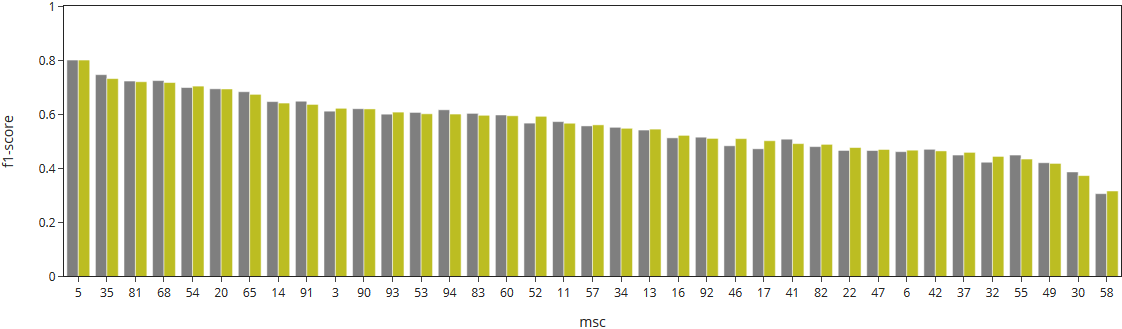
\includegraphics[width=1.1\textwidth]{mathEncoding.png}
  \caption{Effect of mathematical symbols on the encoding.}
\end{figure}

\begin{figure}[h]
  \centering
  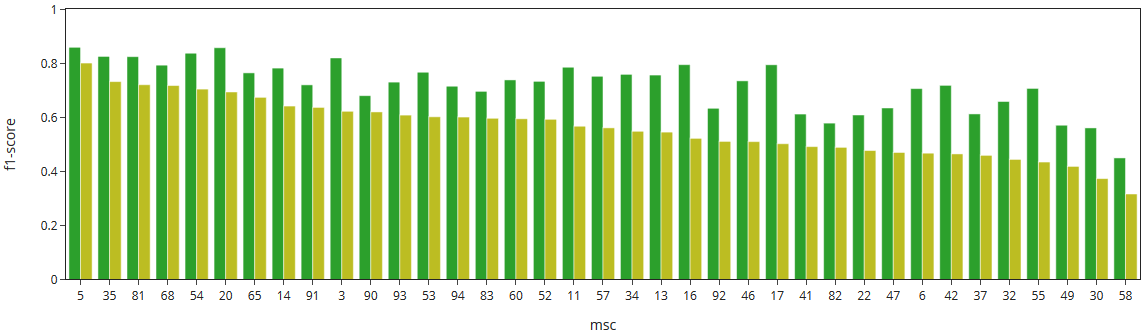
\includegraphics[width=1.1\textwidth]{POSeffekt.png}
  \caption{Effect of POS tagging symbols on the encoding.}
\end{figure}

\begin{figure}[h]
  \centering
  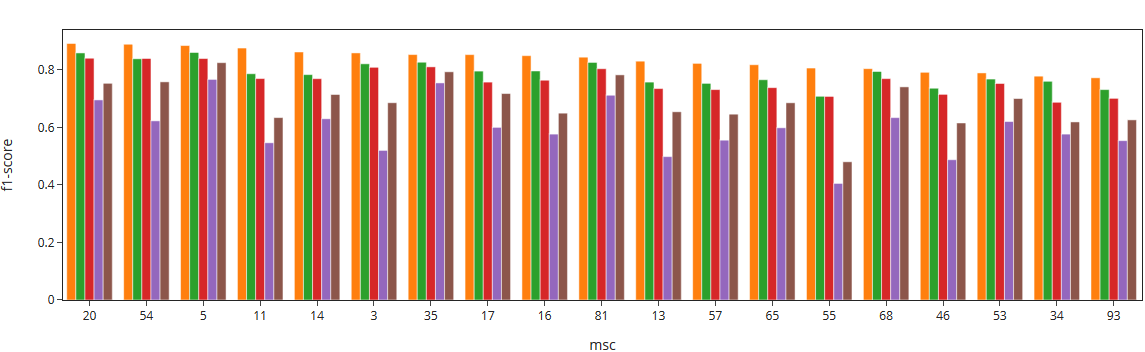
\includegraphics[width=1.1\textwidth]{overview1.png}
  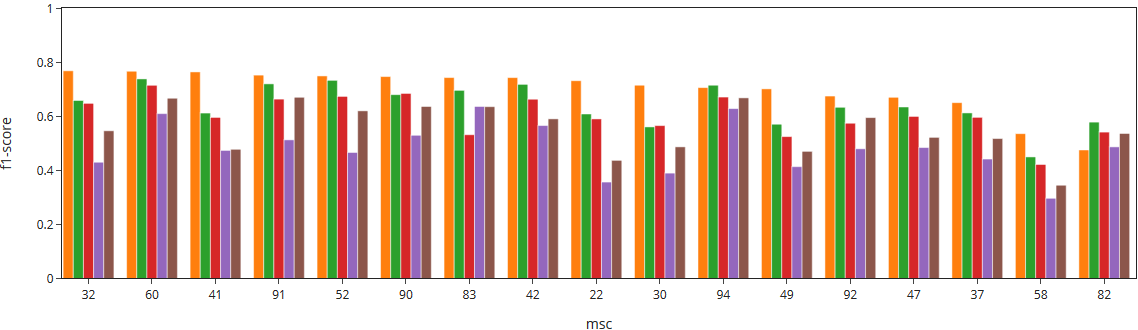
\includegraphics[width=1.1\textwidth]{overview2.png}
  \caption{$F_1$ score of the classification quality of the methods mr1, titer, ref, titls, text grouped by MSC. We use the zbMATH primary MSC as baseline. MSC classes with less than 200 samples were omitted. An interactive version of the figure is available from \url{automsceval.formulasearchengine.com}.}
\end{figure}


\begin{table*}
\begin{tabular}{llll}
  \toprule
  {} &      p &      r &      f \\
  \midrule
  zb1   &      1 &      1 &      1 \\
  mr1   &  0.814 &  0.814 &  0.812 \\
  titer &  0.772 &  0.778 &  0.773 \\
  refs  &  0.748 &  0.753 &  0.746 \\
  titls &  0.637 &  0.627 &  0.623 \\
  texts &  0.699 &  0.709 &  0.699 \\
  ref1  &  0.693 &  0.648 &  0.652 \\
  uT1   &  0.656 &  0.642 &  0.645 \\
  uM1   &  0.655 &  0.639 &  0.644 \\
  tiref &   0.76 &  0.764 &   0.76 \\
  teref &  0.769 &  0.774 &   0.77 \\
  tite  &  0.713 &  0.722 &  0.713 \\
  \bottomrule
\end{tabular}
\begin{tabular}{llll}
  \toprule
  {} &      p &      r &      f \\
  \midrule
  zb1   &  0.817 &  0.807 &   0.81 \\
  mr1   &      1 &      1 &      1 \\
  titer &  0.776 &  0.775 &  0.772 \\
  refs  &  0.743 &  0.743 &  0.737 \\
  titls &  0.644 &  0.632 &  0.627 \\
  texts &  0.704 &  0.709 &  0.699 \\
  ref1  &  0.693 &  0.646 &  0.652 \\
  uT1   &  0.653 &  0.636 &  0.639 \\
  uM1   &  0.652 &  0.632 &  0.636 \\
  tiref &  0.762 &  0.761 &  0.758 \\
  teref &  0.771 &   0.77 &  0.767 \\
  tite  &   0.72 &  0.724 &  0.715 \\
  \bottomrule
\end{tabular}
\caption{Precision $p$, recall $r$ and $F_1$-measure $f$ with regard to the baseline zb1 (left) and mr1 (right).}
\end{table*}


\begin{figure}[h]
  \centering
  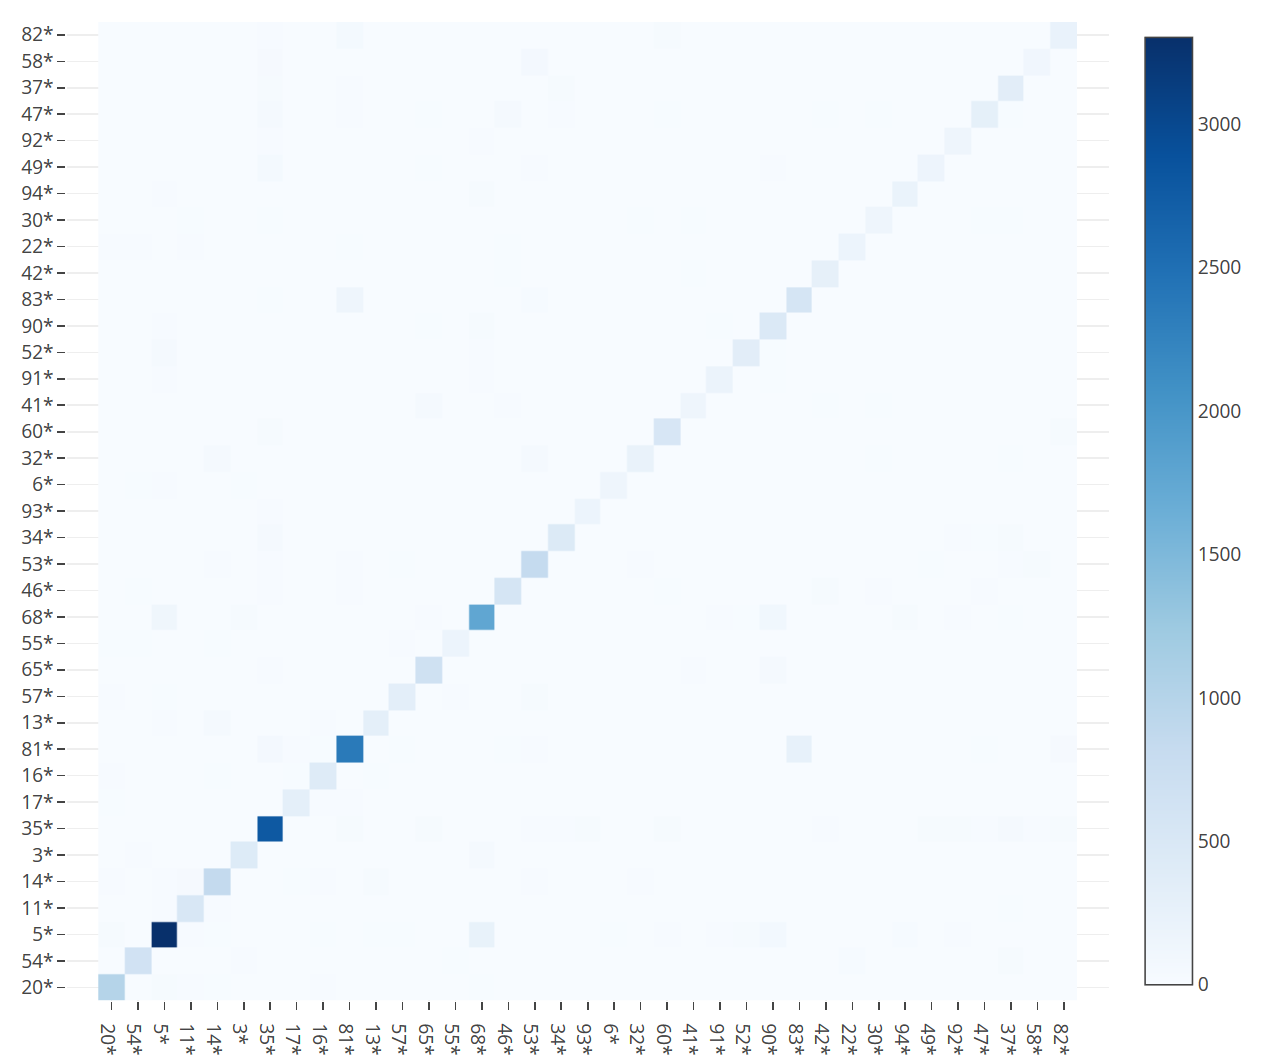
\includegraphics[width=\textwidth]{confusion.png}
  \caption{Confusion matrix (titer).}
\end{figure}

\section{Conclusion \& Future Work}\label{sec.concl}
Regarding the research questions, we summarize our findings as follows:
\begin{enumerate}
  \item The quality of the classification for the coarse grained primary MSC can be evaluated with classical information retrieval methods such as precision, recall and accuracy. The downside of binary evaluation approaches is that the degree of incorrectness is not taken into account. We therefore introduced a non-strict evaluation measure that also counts non-primary MSCs as correct.
  \item We did not find evidence that mathematical expressions improve the coarse grained primary classification.
  \item We found that modern NN such as Bert outperform the POS tagging based model developed by \cite{SchonebergS14}. mathematical expressions improve the coarse grained primary classification.
  \item For most classes the reference based approach outperformed the POS tagged based approach.
  \item The manual classification is significantly better for most classes. 
  \item How to avoid misclassifications in the future?
  \item We consider our current model as good enough for the primary MSC pre classification task. We developed an open API which can be accessed from \url{https://automscbackend.formulasearchengine.com}.
\end{enumerate}

\paragraph{Acknowledgments} This work was supported by the German Research Foundation (DFG grant GI 1259-1).
The authors would like to express their gratitude to Felix Hamborg, and Terry Ruas for their advice in the most recent machine learning technology.
\printbibliography[keyword=primary]